\section{实验结果与分析}\label{sec:experiment}

\subsection{实验环境与设置}

第四章使用 LEVIR-Ship 数据集上已经跑完并能回查的记录，对 DRENet、FCOS 和 YOLO26 进行比较。指标部分保留 AP50、AP50-95、Precision、Recall 与 F1；工程侧另记录 FPS、参数量和 FLOPs。训练配置、权重文件、运行日志和结果文档都单独保存，后续表格、图示和系统演示可以追溯到对应产物。

DRENet 与 YOLO26 的主线实验统一采用 512 输入。FCOS 当前可直接回填的正式结果来自 MMDetection 默认训练口径，输入策略为 1333\(\times\)800。这个差异需要提前说明：DRENet 与 YOLO26 是本文主结论中重点比较的两组结果；FCOS 保留为 anchor-free 参考基线，用于补充检测范式视角，而不用于得出“同输入尺度下严格公平”的结论。

除离线训练和测试外，系统侧真实推理也完成了联调。这样一来，本章的部分分析可以和第五章的任务执行、结果回看等现象对应起来。

\subsection{三模型主对比结果}

三模型核心结果见表~\ref{tab:ch4_baselines}，对应日志和权重均已留存。

\begin{table}[htbp]
  \centering
  \caption{三模型在 LEVIR-Ship 数据集上的主对比结果}
  \label{tab:ch4_baselines}
  \begin{tabular}{lcccccc}
    \toprule
    模型 & AP50 & AP50-95 & Precision & Recall & F1 & 说明 \\
    \midrule
    DRENet & 0.7949 & 0.2919 & 0.4927 & 0.8511 & 0.6241 & 论文主结论模型 \\
    FCOS & 0.7700 & 0.2850 & -- & 0.4050$^{*}$ & -- & anchor-free 参考基线 \\
    YOLO26 & 0.7950 & 0.3170 & 0.8430 & 0.7220 & 0.7778 & 论文主结论模型 \\
    \bottomrule
  \end{tabular}
  \\
  \parbox{0.92\textwidth}{\footnotesize 注：FCOS 当前可直接回填的 0.4050 来自正式 run 中的 \texttt{AR@100} 指标，本文仅用其补充说明检出能力与参考表现，不与 DRENet 和 YOLO26 的 Recall 做严格等值比较。}
\end{table}

\begin{figure}[htbp]
  \centering
  
\includegraphics[width=0.96\textwidth]{img/ch4_main_comparison_chart.png}
  \caption{三模型主对比结果的指标可视化}
  \label{fig:ch4_main_comparison_chart}
\end{figure}

表~\ref{tab:ch4_baselines} 与图~\ref{fig:ch4_main_comparison_chart} 中，YOLO26 和 DRENet 的 AP50 几乎相同，分别为 0.7950 和 0.7949，FCOS 为 0.7700。仅从 AP50 看，专项方法和成熟 one-stage 路线在该数据集上都能完成基本检出，二者差距并不体现在这一项主指标上。

差异主要出现在 AP50-95、Precision 和 Recall 上。YOLO26 的 AP50-95 为 0.3170，高于 DRENet 的 0.2919 和 FCOS 的 0.2850，说明在更严格的 IoU 阈值下，它的边框位置更稳。DRENet 的 Recall 为 0.8511，高于 YOLO26 的 0.7220，但 Precision 只有 0.4927，低于 YOLO26 的 0.8430。也就是说，DRENet 更愿意保留可疑目标，代价是误检更多；YOLO26 对候选框筛选更严格，输出更干净。

FCOS 的 AP50 和 AP50-95 均低于前两者。在当前实验条件下，通用 anchor-free 基线没有表现出优势。不过 FCOS 仍有保留意义：它给后文讨论专项设计和 one-stage 部署路线时提供了另一条参照线。

\subsection{效率与部署属性分析}

除精度指标外，工程部署场景还要关注模型在速度和复杂度方面的表现。当前可用效率结果如表~\ref{tab:ch4_efficiency} 所示。

\begin{table}[htbp]
  \centering
  \caption{三模型效率与复杂度对比}
  \label{tab:ch4_efficiency}
  \small
  \begin{tabular}{lccccl}
    \toprule
    模型 & FPS & Params(M) & FLOPs(G) & 输入尺寸 & 说明 \\
    \midrule
    DRENet & 121.8993 & 4.7882 & 4.2057 & 512 & 同口径效率测试 \\
    FCOS & 45.9559 & 32.1664 & 123.0 & 1333\(\times\)800 & 输入策略不同，仅作参考 \\
    YOLO26 & 69.0625 & 2.5042 & 3.6939 & 512 & 同口径效率测试 \\
    \bottomrule
  \end{tabular}
\end{table}

效率表中的趋势和精度表并不完全相同。DRENet 在当前记录中 FPS 最高，说明在本文的测试环境和测量方式下，它的推理速度较突出。YOLO26 的参数量为 2.5042M、FLOPs 为 3.6939G，模型规模更小。FCOS 采用不同输入策略和实现框架，其效率数值更适合作为历史正式 run 的参考成本，不宜直接和前两者做严格同口径比较。

把精度和效率放在一起读，DRENet 更适合漏检敏感的目标排查场景。YOLO26 更适合作为默认系统模型，因为它在定位质量、误检控制、模型规模和接口封装上更均衡。FCOS 仍是补充参考，不作为系统默认主模型。

\subsection{模型逐项分析}

\subsubsection{DRENet 结果分析}

DRENet 在本文结果中最醒目的特点是 Recall 高。当前正式结果中，它的 Recall 为 0.8511，高于 YOLO26，说明该模型在复杂背景和弱纹理目标上更倾向于保留候选框。若任务目标是先尽可能发现可疑船舶，再由后续流程复核，这种取向有实际价值。

DRENet 的问题也很直接：Precision 为 0.4927，误检压力较大。近岸区域、港区设施和背景边缘纹理都可能被它保留下来。因此，DRENet 更适合作为召回优先的候选方案；若要进入更严格的部署流程，还需要通过阈值、后处理或融合策略继续压低误检。

\subsubsection{FCOS 结果分析}

FCOS 的 AP50 为 0.7700，低于 DRENet 与 YOLO26。在当前中分辨率遥感微小船舶任务中，通用 anchor-free 路线没有占到优势。另需说明，表~\ref{tab:ch4_baselines} 中 FCOS 的 0.4050 来自正式 run 的 \texttt{AR@100}，并不是与 DRENet、YOLO26 完全等价的标准 Recall。本文引用它，只是为了补充 FCOS 的检出能力范围。

FCOS 的价值不在单点最优，而在于它结构清晰、范式明确。保留这组结果后，专项设计和 one-stage 路线在该任务中的差异更容易讨论。

\subsubsection{YOLO26 结果分析}

YOLO26 的 AP50 与 DRENet 基本持平，但 AP50-95、Precision 和 F1 更高。Precision 达到 0.8430，说明在当前阈值设置下，它对复杂背景中的伪目标压制更强，输出框更少出现大面积冗余。

工程侧也更偏向 YOLO26。它的训练链路较成熟，接口封装直接，接入系统时需要处理的特殊情况较少。若从默认模型角度选择，YOLO26 的竞争力更强；与 DRENet 配合时，它也可以在误检控制上形成互补。

\subsection{定性样例与误差分析}

定量指标只能给出整体趋势，不能直接说明模型在某张图上为什么错。为便于解释，本文从系统导出的可视化结果中整理成功检测、漏检和误检样例。样例按“模型 $\rightarrow$ 场景类型”归档，后续论文插图和答辩展示使用同一批文件。

\subsubsection{成功检测样例}

成功样例中，DRENet 在海面纹理较弱、目标尺寸较小的图像上仍能给出响应，这与它召回偏高的定量结果相符。YOLO26 的结果更整洁，尤其在多目标和常规场景中，预测框与标注框的匹配更稳定。FCOS 也能在部分样例中完成定位，但波动更大。图~\ref{fig:ch4_success_cases} 使用“列为模型、行为 Label/Prediction”的统一布局，展示各模型的代表样本。

\begin{figure}[htbp]
  \centering
  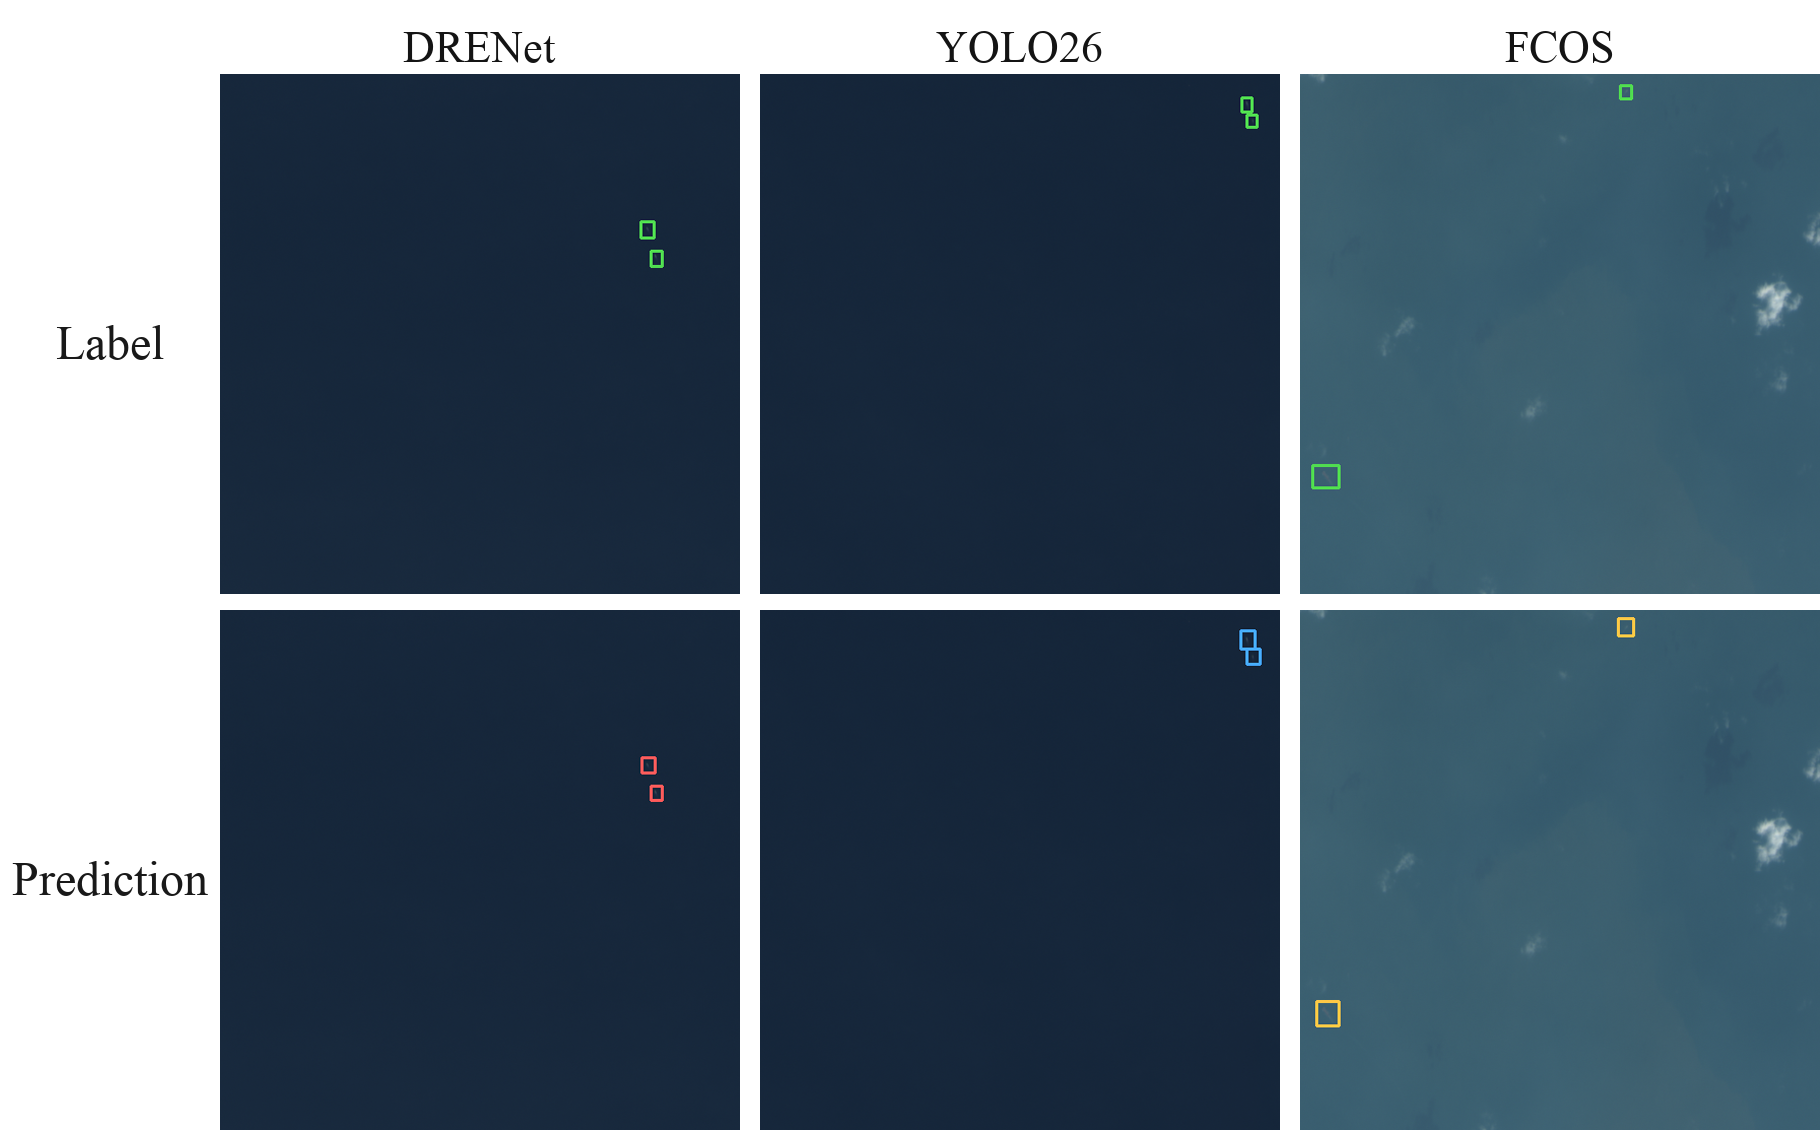
\includegraphics[width=0.95\textwidth]{img/ch4_success_cases.png}
  \caption{三模型成功检测样例对比}
  \label{fig:ch4_success_cases}
\end{figure}

\subsubsection{漏检样例}

漏检样例中，三类模型都会遗漏目标，但遗漏位置和原因不完全相同。图~\ref{fig:ch4_miss_cases} 同样采用“列为模型、行为 Label/Prediction”的排布方式，对比标注框和预测框之间的缺失。弱纹理、小尺寸以及背景对比度不足，是这些漏检样例中反复出现的因素。

\begin{figure}[htbp]
  \centering
  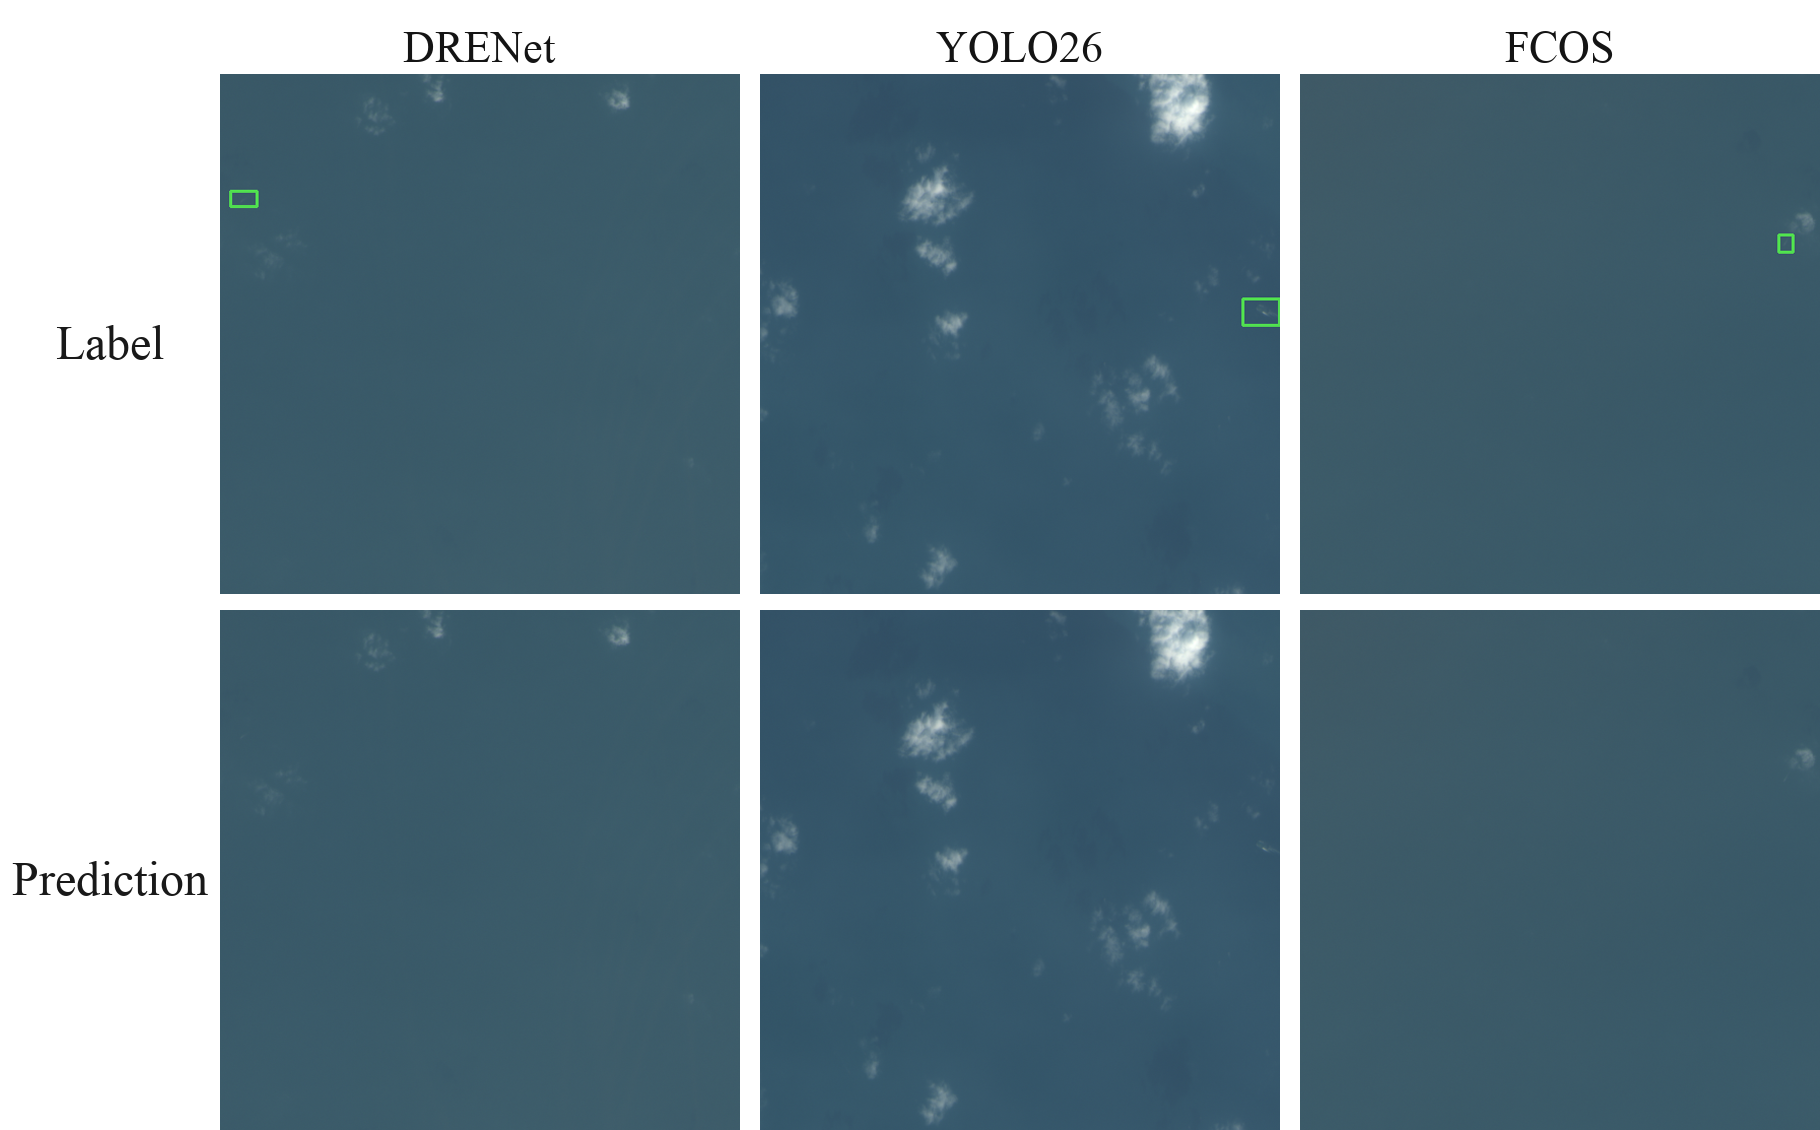
\includegraphics[width=0.95\textwidth]{img/ch4_miss_cases.png}
  \caption{三模型漏检样例对比}
  \label{fig:ch4_miss_cases}
\end{figure}

\subsubsection{误检样例}

误检样例则更能解释 Precision 差异。DRENet 更容易把复杂背景纹理保留下来；YOLO26 偶尔会在边缘背景区域产生额外响应；FCOS 也存在误检，但数量和位置与前两者不同。图~\ref{fig:ch4_false_positive_cases} 用统一版式展示模型独立样本，便于对比误检来源。

\begin{figure}[htbp]
  \centering
  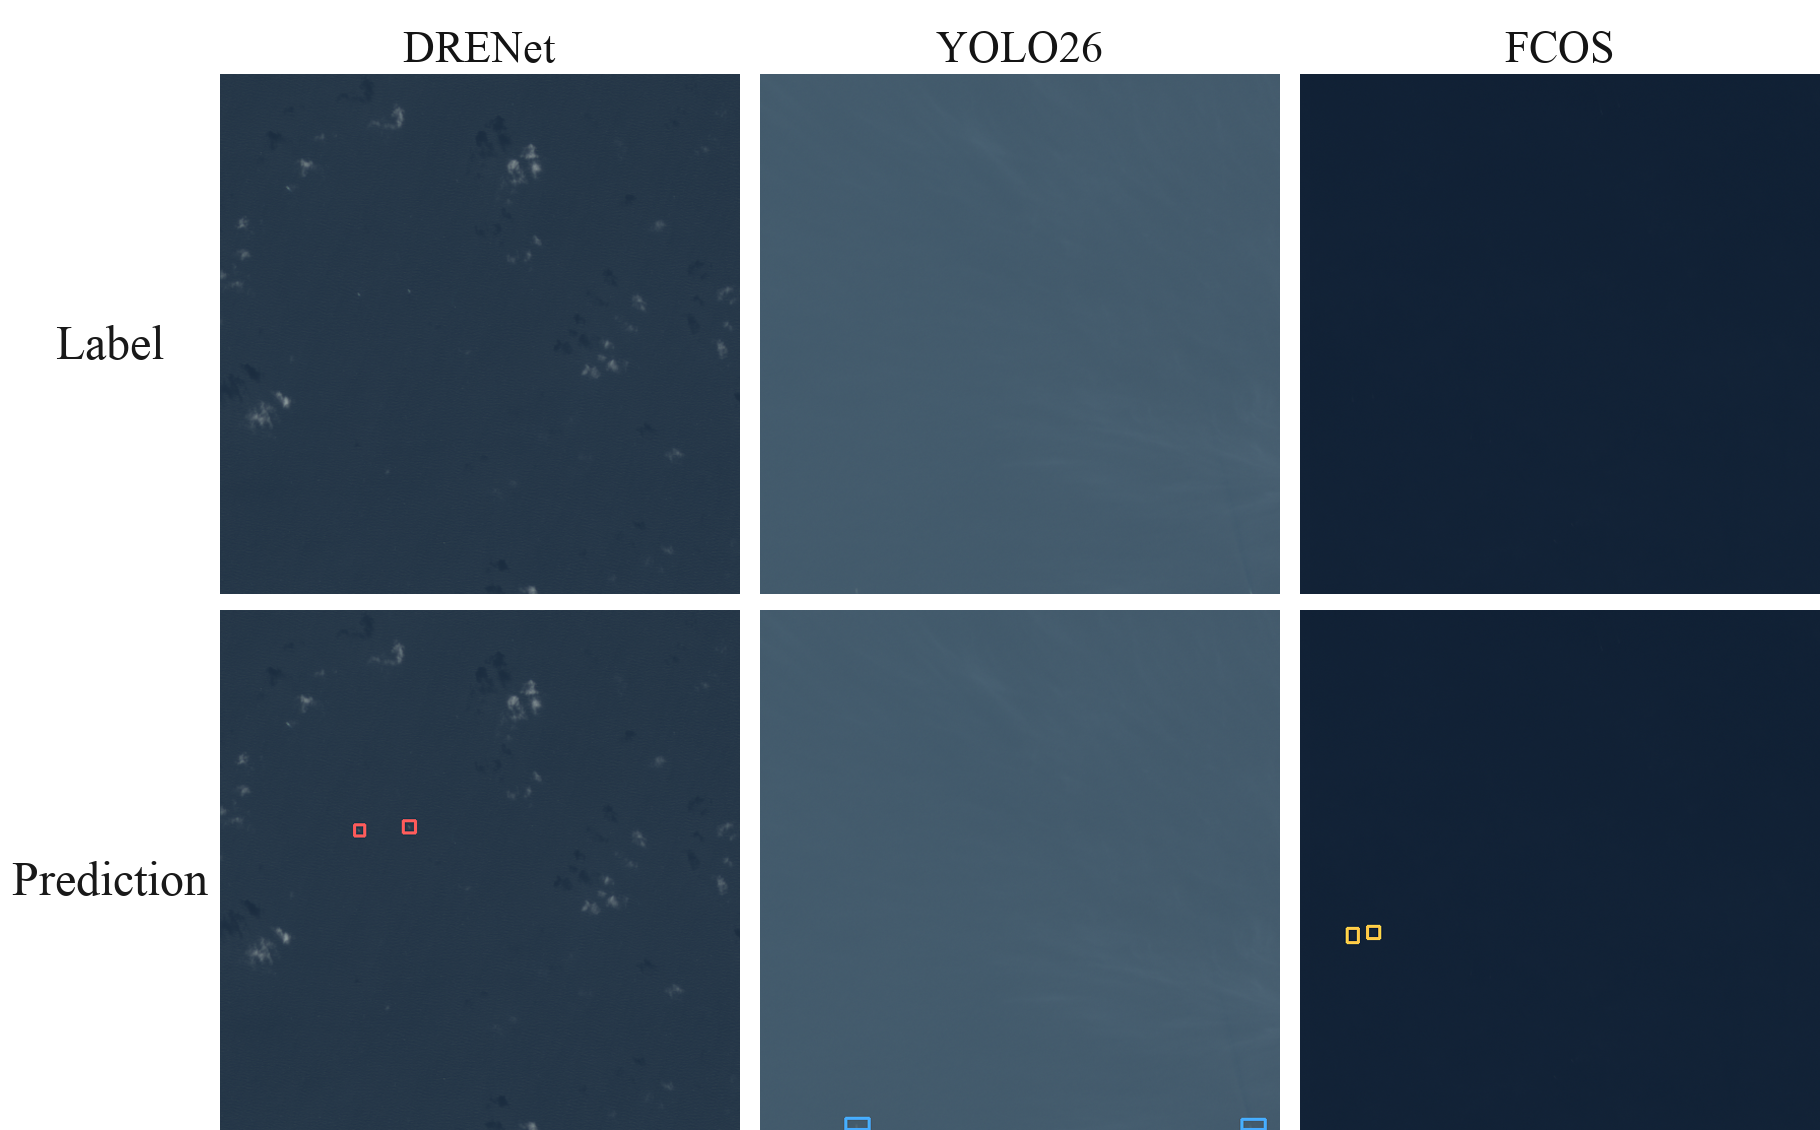
\includegraphics[width=0.95\textwidth]{img/ch4_false_positive_cases.png}
  \caption{三模型误检样例对比}
  \label{fig:ch4_false_positive_cases}
\end{figure}

把这些样例和表~\ref{tab:ch4_baselines} 对照后可以发现，DRENet 与 YOLO26 的差别并不是单纯分数高低。DRENet 更偏向“先检出”，复杂背景下误检会变多；YOLO26 更偏向输出稳定和边框质量，弱目标场景下可能漏掉一部分目标。FCOS 则继续作为 anchor-free 路线的补充参照。

\subsection{消融实验}

为了说明主表中 Precision 与 Recall 的差异，实验部分补充了两组离线消融。第一组固定 IoU 阈值，只改变置信度阈值，观察候选框筛选松紧变化后各模型的响应。第二组不重新训练模型，只在推理阶段改输入尺寸，用来查看现有权重面对尺度扰动时的表现。后一组不是严格的训练尺度消融，主要用于行为解释。

\subsubsection{阈值消融分析}

阈值消融固定 IoU 阈值为 0.50，置信度阈值取 0.15、0.25 和 0.35。本文主要关心两个问题：阈值升高后，Precision 和 Recall 是否按预期方向变化；系统默认使用 0.25 是否有实验依据。FCOS 在本节使用系统联调和离线复算所采用的稳定候选 checkpoint，不使用主对比表中的历史最佳单点结果。三模型结果见表~\ref{tab:ch4_threshold_ablation}。

\begin{table}[htbp]
  \centering
  \small
  \caption{三模型阈值消融结果}
  \label{tab:ch4_threshold_ablation}
  \begin{tabular}{@{}llccccp{4.2cm}@{}}
    \toprule
    模型 & 设置 & AP50 & Precision & Recall & F1 & 结论 \\
    \midrule
    DRENet & conf=0.15 & 0.6616 & 0.6441 & 0.7935 & 0.7110 & 低阈值召回更高，但误检增加 \\
    DRENet & conf=0.25 & 0.6616 & 0.7331 & 0.7663 & 0.7493 & 默认值更均衡 \\
    DRENet & conf=0.35 & 0.6616 & 0.7778 & 0.7355 & 0.7561 & 精度继续上升，召回下降 \\
    FCOS & conf=0.15 & 0.7389 & 0.7283 & 0.8351 & 0.7781 & 低阈值检出更充分 \\
    FCOS & conf=0.25 & 0.7389 & 0.7621 & 0.8297 & 0.7944 & 默认值已较均衡 \\
    FCOS & conf=0.35 & 0.7389 & 0.7761 & 0.8225 & 0.7986 & F1 略优于 0.25 \\
    YOLO26 & conf=0.15 & 0.6661 & 0.6412 & 0.7899 & 0.7078 & 召回提升明显，但误检偏多 \\
    YOLO26 & conf=0.25 & 0.6661 & 0.7527 & 0.7609 & 0.7568 & 综合表现最均衡 \\
    YOLO26 & conf=0.35 & 0.5914 & 0.8248 & 0.6993 & 0.7569 & 精度最高，但 AP50 与召回下降 \\
    \bottomrule
  \end{tabular}
\end{table}

\begin{figure}[htbp]
  \centering
  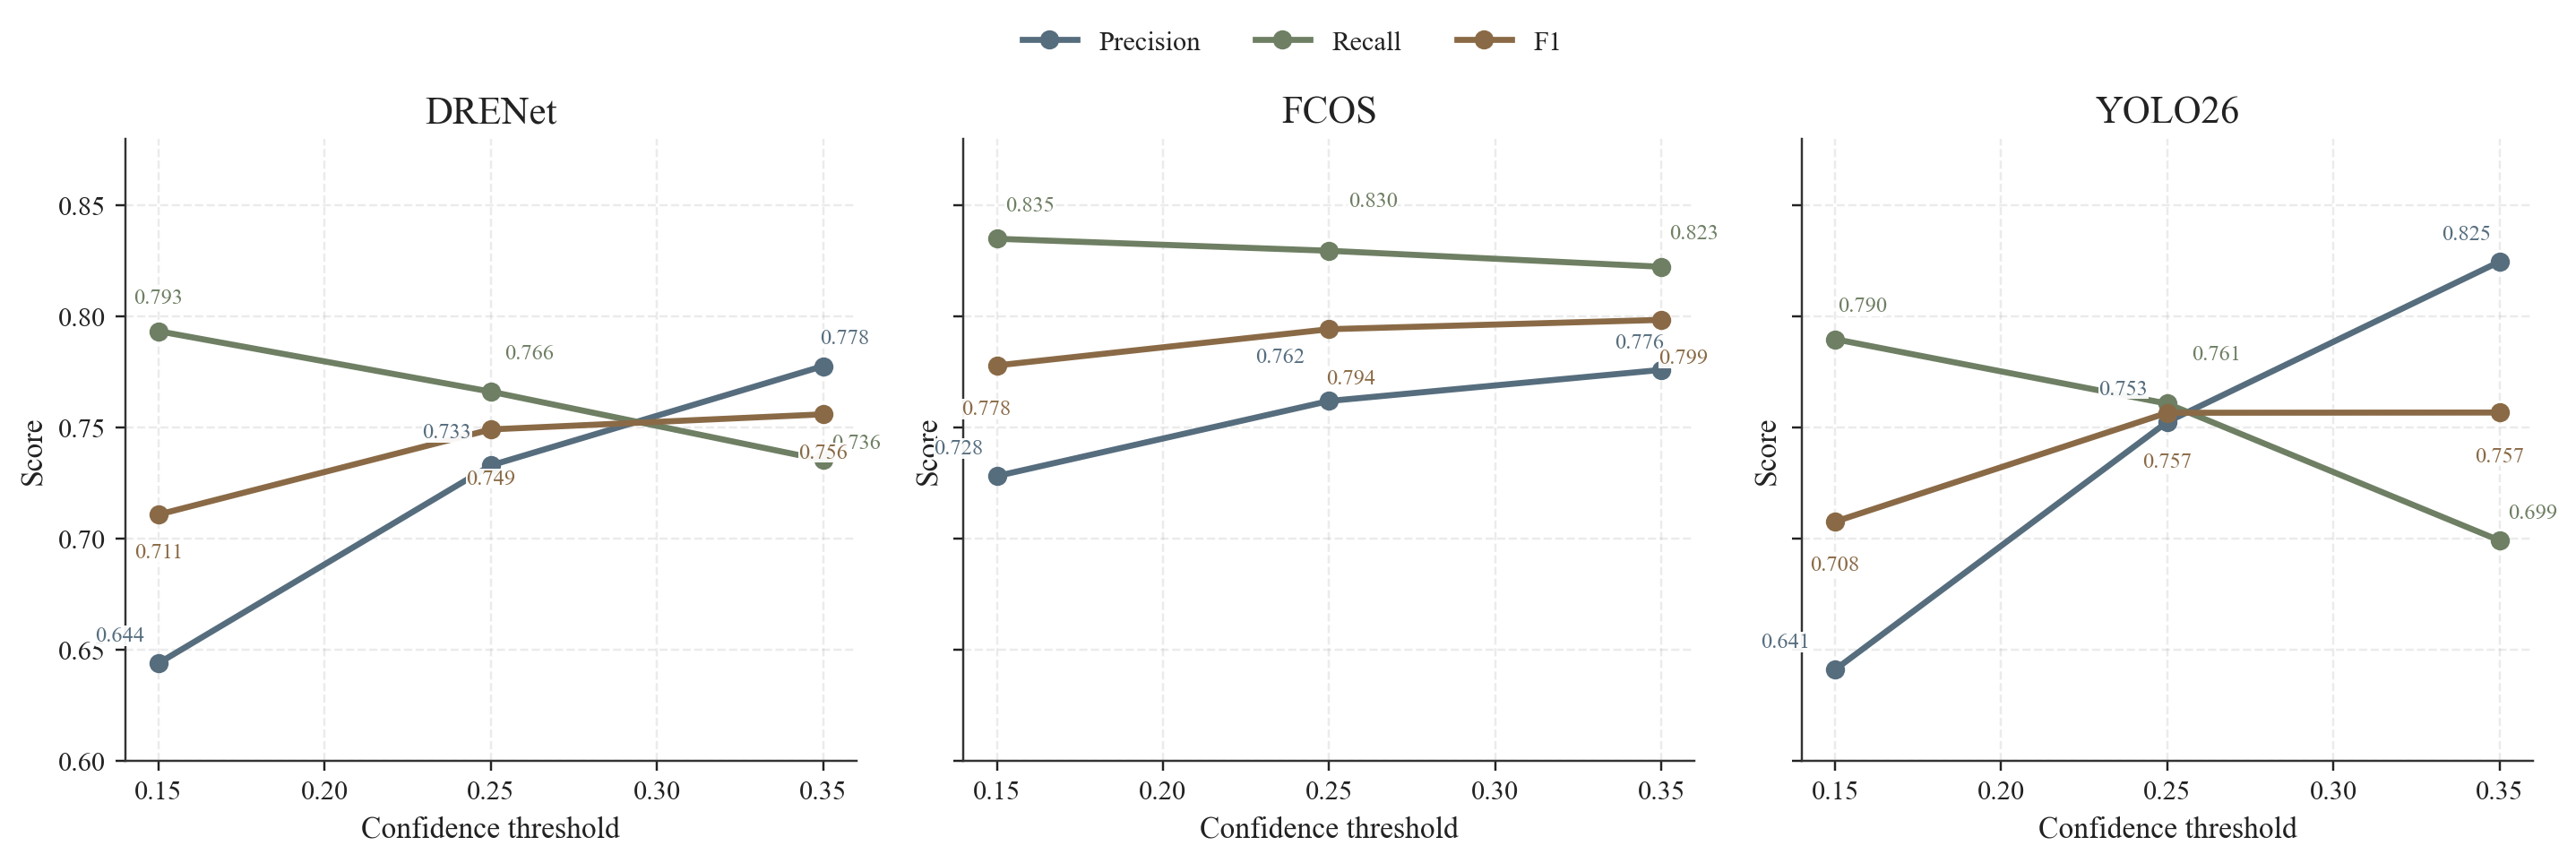
\includegraphics[width=0.98\textwidth]{img/ch4_threshold_trend.png}
  \caption{三模型阈值消融趋势图}
  \label{fig:ch4_threshold_trend}
\end{figure}

表~\ref{tab:ch4_threshold_ablation} 和图~\ref{fig:ch4_threshold_trend} 显示，阈值升高后，三模型的 Precision 大多上升，Recall 大多下降。这一趋势符合候选框筛选逻辑，也说明后处理阈值会明显改变遥感微小船舶检测结果。

DRENet 对阈值较敏感。低阈值会进一步放大它的召回倾向，但误检也随之增加；阈值提高到 0.35 后，Precision 升至 0.7778，Recall 降至 0.7355。若系统需要在检出率和误检数量之间取一个中间位置，0.25 比 0.15 和 0.35 更适合作为默认值。

FCOS 和 YOLO26 的变化则更细。FCOS 在当前稳定权重下，阈值由 0.25 提高到 0.35 时，F1 从 0.7944 小幅升至 0.7986，说明这组权重下略高阈值能压掉一部分冗余候选。YOLO26 在 0.25 时 AP50、Precision 和 Recall 的组合更均衡；继续升到 0.35 后，Precision 到 0.8248，但 AP50 与 Recall 同时下降。因此，系统默认参数仍采用 0.25，解释和演示都更稳。

\subsubsection{输入尺寸敏感性分析}

输入尺寸敏感性分析关注推理阶段放大目标后模型会怎样变化。本组实验不重新训练，只覆写推理输入尺寸，所以它反映的是现有权重面对尺度扰动时的行为，而不是训练尺度消融。FCOS 主对比参考结果来自历史正式 run 的最佳点；本节尺寸分析基于稳定候选 checkpoint 离线复算。因此，这里的数值只用于解释趋势，不反向改写前文主表结论。YOLO26 与 FCOS 的结果见表~\ref{tab:ch4_size_ablation}。

\begin{table}[htbp]
  \centering
  \small
  \caption{输入尺寸敏感性分析结果}
  \label{tab:ch4_size_ablation}
  \begin{tabular}{@{}llccccp{4.2cm}@{}}
    \toprule
    模型 & 设置 & AP50 & Precision & Recall & F1 & 结论 \\
    \midrule
    FCOS & imgsz=512 & 0.4490 & 0.5903 & 0.6395 & 0.6139 & 输入过小，性能明显受限 \\
    FCOS & imgsz=640 & 0.6452 & 0.7405 & 0.7808 & 0.7601 & 相比 512 提升显著 \\
    FCOS & imgsz=800 & 0.7389 & 0.7621 & 0.8297 & 0.7944 & 当前组内最佳 \\
    YOLO26 & imgsz=512 & 0.6661 & 0.7527 & 0.7609 & 0.7568 & 基线稳定 \\
    YOLO26 & imgsz=640 & 0.6737 & 0.7543 & 0.7953 & 0.7743 & 当前组内最均衡 \\
    YOLO26 & imgsz=800 & 0.6564 & 0.6827 & 0.7989 & 0.7362 & 召回升高，但精度下降 \\
    \bottomrule
  \end{tabular}
\end{table}

\begin{figure}[htbp]
  \centering
  
\includegraphics[width=0.96\textwidth]{img/ch4_size_trend.png}
  \caption{输入尺寸敏感性趋势图}
  \label{fig:ch4_size_trend}
\end{figure}

表~\ref{tab:ch4_size_ablation} 与图~\ref{fig:ch4_size_trend} 中，FCOS 对输入尺寸变化非常敏感。输入由 512 提到 640 后，AP50 从 0.4490 升至 0.6452，F1 从 0.6139 升至 0.7601；继续到 800 后，AP50 和 F1 分别达到 0.7389 与 0.7944。这说明当前 FCOS 权重较依赖更大的推理输入，目标被放大后，候选生成和定位都更容易。

YOLO26 的曲线不同。它在 640 输入下取得本组最佳 AP50 和 F1；当尺寸继续增至 800 时，Recall 从 0.7953 小幅升至 0.7989，但 Precision 明显下降，F1 也降低。由此可以判断，YOLO26 在更大输入下会发现更多候选目标，同时也更容易引入误检。对 YOLO26 来说，输入尺寸不是越大越好。

DRENet 未放入本组尺寸主表，是因为当前本地插件路径在非 512 输入下会触发结构 shape mismatch，640 和 800 设置无法稳定输出。本文把它写为实现边界，而不是简单写作“实验不足”。这种表述能和第五章对本地插件约束的说明保持一致。

另外，本文曾在 20 张图子样本上做过 \texttt{smoke\_limit} 检查。该检查只用于确认尺寸趋势在小样本上没有反向，不进入正文主表，以免和全量测试集结果混用。

\subsection{系统口径与论文口径说明}

论文主表、消融实验和系统演示使用的模型口径并不完全相同，本文在这里单独说明。主结论重点使用 DRENet 与 YOLO26 的正式结果，FCOS 作为参考基线保留；系统实现中除单模型推理外，还提供融合模式和默认权重配置。对于 FCOS，本文区分“论文主对比口径”和“系统与消融口径”：前者对应历史正式 run 中用于主表展示的最佳离线结果，后者对应系统联调、定性导出和离线消融所使用的稳定候选 checkpoint。

这样的区分不是把论文和系统割裂开，而是把不同结果的用途说清楚。论文主表更重视结论解释和正式记录；系统更重视任务执行稳定性与展示效果；消融实验则用于观察统一复算条件下的参数扰动。答辩时若遇到不同表格和系统结果来源的问题，可以按这个口径解释。

\subsection{当前边界与改进方向}

目前实验部分还有几处边界。第一，输入尺寸敏感性分析只覆盖 YOLO26 与 FCOS；DRENet 的本地插件在非 512 输入下会触发 shape mismatch，所以这里只保留实现边界说明。第二，FCOS 的效率结果与正式参考结果使用的输入策略不同，只能作为参考值。第三，融合模式已经能稳定运行，但尚未形成统一离线 AP 主表，因此不放入主结论。

这些边界不改变本文的主线判断：DRENet 与 YOLO26 的正式结果已经支撑主要对比，FCOS 的参考角色也已经限定。后续若继续完善，可优先补充融合模式离线 AP、同口径效率测试，以及 FCOS 同尺度训练复现。

\subsection{小结}

本章整理了 DRENet、FCOS 和 YOLO26 的定量结果、误差样例和消融结果。整体判断是：DRENet 更偏召回，YOLO26 在精度、误检控制和部署接入上更均衡，FCOS 保留为 anchor-free 参照。第五章继续说明这些模型结果如何进入系统任务流程。
